\subsection{Budget-neutral swaps in simulations and agricultural data}\label{res:swaps}

Appendix Table~\ref{tab:swap_simulation} compares policies over 500 replications for each simulation
design. Under weak overlap and heterogeneous effects, robust swaps lose to the exposure
reference in 29.0 per cent of test samples, compared with 40.6 per cent for DR swaps and
35.8 per cent for plug-in swaps. Their mean gain is 0.0096, compared with 0.0053 and 0.0078.
The paired mean gains of robust over DR and plug-in are 0.0044 (Monte Carlo SE 0.0010)
and 0.0018 (SE 0.0009), respectively. Mean-score swaps lose in 36.2 per cent of
weak-overlap draws. The paired gain of robust over mean-score swaps is 0.0016
(SE 0.0009). The mean-gain comparisons with plug-in and mean-score swaps are small
relative to their Monte Carlo uncertainty. Under moderate overlap, mean-score swaps
have a slightly lower loss rate than robust swaps (26.8 against 27.2 per cent).
When effects are homogeneous, all fitted methods have negative mean gains. Robust
swaps underperform the exposure reference in 87.0 per cent of these replications.

In the five country folds, robust swaps replace 21 of 37 places and have an estimated
gain of 0.455 (conditional 95 per cent interval $[-0.122,1.219]$). With 0.05 clipping
in the evaluation score, the estimate is 0.432 ($[-0.147,1.187]$). Holding out entire
regions changes which countries are compared and which model is used to score them.
The robust rule replaces 14 of 37 places and has an estimated gain of 0.065
($[-0.184,0.403]$), or 0.067 ($[-0.175,0.399]$) with the alternative clipping.
DR, plug-in and mean-score swaps have higher point estimates in the regional
exercise. In the country folds their point estimates are all at or below zero.
The comparisons give no reliable evidence that robust swaps improve on the
exposure ranking in the agricultural sample. They do demonstrate that model choice
and the comparison population can change the assessment even under an exact quota.

\subsection{Ellipsoidal portfolio risk and held-out welfare}\label{res:ellipsoid}

Figure~\ref{fig:simulation_tradeoff} reports results from 600 independent test evaluations.
Under weak overlap, the ellipsoidal portfolio loses to the reference in 3.5 per
cent of replications, against 26.5 per cent for threshold swaps and 22.5 per cent
for ranking the pooled means. Its paired average gain over threshold swaps is
0.00527 (Monte Carlo SE 0.00137). Its mean gain is virtually the same as that
of the pooled-mean rule. With moderate overlap, paying for protection reduces
mean gain by 0.00448 relative to pooling alone (SE 0.00137) and lowers the loss
rate from 18.5 to 5.0 per cent. When the true effects are homogeneous the
reference is optimal. The penalty reduces mean losses from 0.0206 under the
pooled-mean policy to 0.0021, and reduces but does not eliminate the risk of
making unnecessary exchanges.

\begin{figure}[htbp]
\centering
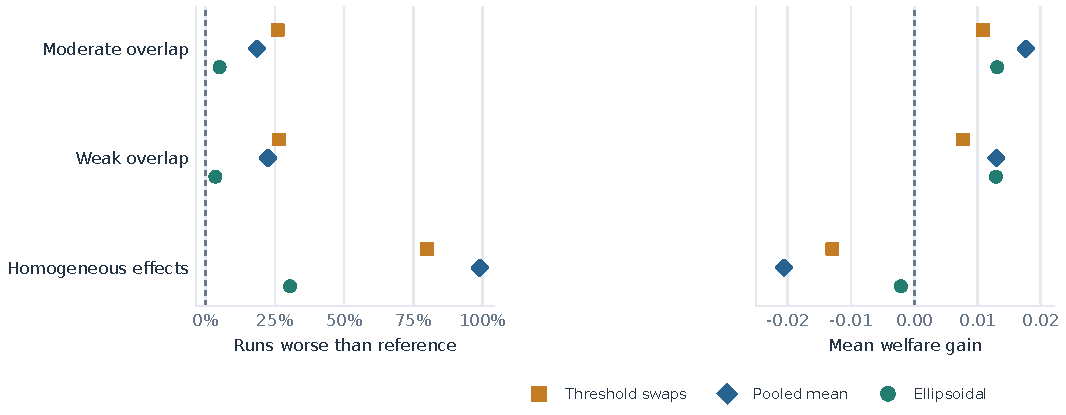
\includegraphics[width=\linewidth]{simulation_tradeoff.pdf}
\caption{Risk and mean welfare in the ellipsoidal portfolio simulations, using 200 replications per design. A loss occurs when a policy underperforms the exposure reference. Both measures are relative to that reference, which has zero gain and zero loss rate by construction. See Appendix Table~\ref{tab:ellipsoid_simulation} for full results.}
\label{fig:simulation_tradeoff}
\end{figure}

The solver reaches the stated total-gain tolerance of $10^{-5}$ in 591 of the
600 simulations under finite solve limits. Across all replications the worst
remaining gap in mean gain per test country is below $0.00082$. All 12
agricultural batches reach the tolerance. Their largest remaining gap in
mean gain per country is approximately $1.1\times10^{-7}$.

In held-out country folds the ellipsoidal portfolio replaces seven places and
has an estimated gain of $-0.271$ (conditional 95 per cent interval
$[-0.754,-0.009]$, Figure~\ref{fig:heldout_welfare}). The estimate is
$-0.256$ with propensity clipping at 0.05. For whole-region holdouts it retains
the reference in every batch. The small solver gaps rule out incomplete
numerical optimisation as an explanation for weak held-out welfare. The
ellipsoid represents uncertainty in fitted changes in heat sensitivity. It
does not resolve the limitations of the research proxy, prediction across
regions, or the uncertainty of using the data to choose a portfolio. The
simulation results show a risk--return trade-off in the specified designs.
The application gives little reason to change an exposure-based ranking
on the available evidence.

\begin{figure}[htbp]
\centering
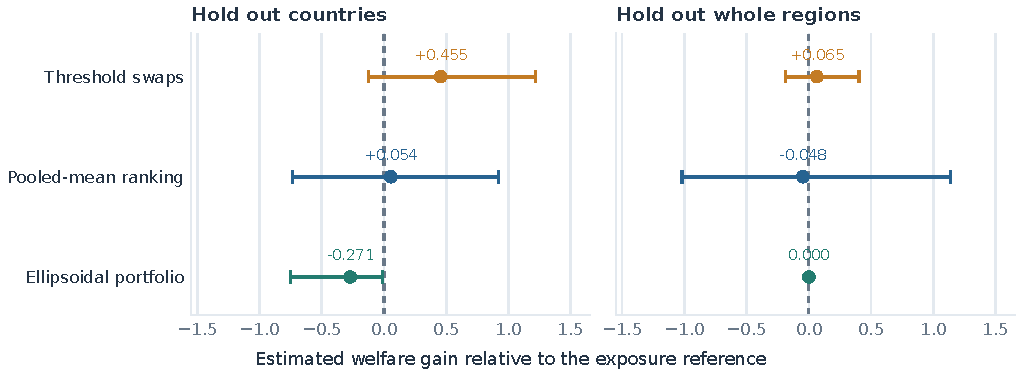
\includegraphics[width=\linewidth]{heldout_welfare.pdf}
\caption{Estimated welfare gains over the exposure reference on held-out countries and whole regions. Each method allocates exactly 37 places. Bars show conditional bootstrap 95\% intervals with the fitted rules and scores held fixed. The ellipsoidal rule retains the reference in the region folds, so its gain and interval are zero by construction. See Appendix Table~\ref{tab:ellipsoid_application} for numerical results.}
\label{fig:heldout_welfare}
\end{figure}

\subsection{Exchange-grid solver benchmark}\label{res:exchange_grid}

\begin{figure}[htbp]
\centering
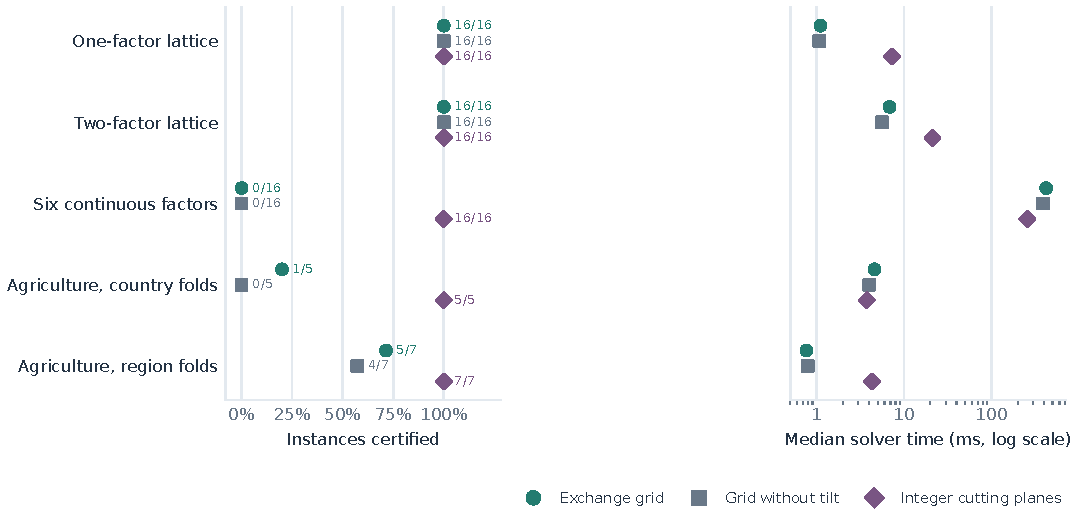
\includegraphics[width=\linewidth]{solver_benchmark.pdf}
\caption{Solver certificates and median runtime across five designs. Fractions in the left panel show the number of instances meeting the total-gain gap tolerance of $10^{-5}$. The right panel reports milliseconds on a log scale for all instances, including runs that stop before certification. Times are specific to this machine. See Appendix Table~\ref{tab:exchange_grid} for the counts.}
\label{fig:solver_benchmark}
\end{figure}

On the one- and two-factor lattices the exchange-grid method certifies every
instance and attains the same objective as the integer cutting-plane solver.
Its median runtime is about one sixth and one third of that solver's,
respectively, on this machine. Both grid variants use the same exact
recurrence on these inputs. The speed comparisons therefore measure the
benefit of the lattice recurrence. Neither grid variant closes the gap on the
six-continuous-factor design. The tilt comparison isolates the benefit of
accounting for omitted directions. The median gap falls from 3.811 to 3.300,
while integer cutting planes certify every instance. On the
agricultural objectives the tilted grid certifies six of 12 batches, against
four for the untilted grid and 12 for integer cutting planes. The new
recurrence is competitive on small discrete risk signatures. Integer cutting
planes provide stronger certificates on the fitted agricultural problems,
so the agricultural welfare comparisons in Section~\ref{res:ellipsoid}
continue to use those solutions.
